% Use only LaTeX2e, calling the article.cls class and 12-point type.

\documentclass[12pt]{article}

\makeatletter
\renewcommand\paragraph{\@startsection{paragraph}{4}{\z@}%
            {-2.5ex\@plus -1ex \@minus -.25ex}%
            {1.25ex \@plus .25ex}%
            {\normalfont\normalsize\bfseries}}
\makeatother
\setcounter{secnumdepth}{4} % how many sectioning levels to assign numbers to

% Users of the {thebibliography} environment or BibTeX should use the
% scicite.sty package, downloadable from *Science* at
% www.sciencemag.org/about/authors/prep/TeX_help/ .
% This package should properly format in-text
% reference calls and reference-list numbers.

%\usepackage{scicite}

% Use times if you have the font installed; otherwise, comment out the
% following line.

\usepackage{times}
\usepackage{amsmath}
\usepackage{graphicx}
\usepackage{subfig}
\usepackage{float}

% The preamble here sets up a lot of new/revised commands and
% environments.  It's annoying, but please do *not* try to strip these
% out into a separate .sty file (which could lead to the loss of some
% information when we convert the file to other formats).  Instead, keep
% them in the preamble of your main LaTeX source file.


% The following parameters seem to provide a reasonable page setup.

\topmargin 0.0cm
\oddsidemargin 0.2cm
\textwidth 16cm 
\textheight 21cm
\footskip 1.0cm


%The next command sets up an environment for the abstract to your paper.

\newenvironment{sciabstract}{%
\begin{quote} \bf}
{\end{quote}}


% The following lines set up an environment for the last note in the
% reference list, which commonly includes acknowledgments of funding,
% help, etc.  It's intended for users of BibTeX or the {thebibliography}
% environment.  Users who are hand-coding their references at the end
% using a list environment such as {enumerate} can simply add another
% item at the end, and it will be numbered automatically.

\newcounter{lastnote}
\newenvironment{scilastnote}{%
\setcounter{lastnote}{\value{enumiv}}%
\addtocounter{lastnote}{+1}%
\begin{list}%
{\arabic{lastnote}.}
{\setlength{\leftmargin}{.22in}}
{\setlength{\labelsep}{.5em}}}
{\end{list}}


% Include your paper's title here

\title{Invaders on Daisyworld:\\ A Computer Simulation of Invasive Species}


% Place the author information here.  Please hand-code the contact
% information and notecalls; do *not* use \footnote commands.  Let the
% author contact information appear immediately below the author names
% as shown.  We would also prefer that you don't change the type-size
% settings shown here.

\author{
  Jack Hosemans\\
  \normalsize{jmhos3@student.monash.edu}\\
  \\
  \normalsize{Faculty of Information Technology}\\
  \normalsize{Monash University, Clayton, Australia}
}

% Include the date command, but leave its argument blank.

\date{}



%%%%%%%%%%%%%%%%% END OF PREAMBLE %%%%%%%%%%%%%%%%



\begin{document} 

% Double-space the manuscript.
\baselineskip24pt

% Make the title.

\maketitle 

{\bf \quad Keywords:} TODO

% Place your abstract within the special {sciabstract} environment.

\begin{sciabstract}
ABSTRACT GOES HERE TODO
\end{sciabstract}



% In setting up this template for *Science* papers, we've used both
% the \section* command and the \paragraph* command for topical
% divisions.  Which you use will of course depend on the type of paper
% you're writing.  Review Articles tend to have displayed headings, for
% which \section* is more appropriate; Research Articles, when they have
% formal topical divisions at all, tend to signal them with bold text
% that runs into the paragraph, for which \paragraph* is the right
% choice.  Either way, use the asterisk (*) modifier, as shown, to
% suppress numbering.

\section{Introduction}
A healthy ecosystem exhibits homeostatic properties\cite{morgan2001}
that maintain an environment hospitable to the native species,
allowing for a stable system in situations where life may not normally
exist. External pressures such as climate change may cause an
ecosystem to collapse given there is a large enough change that the
system cannot react in time\cite{barry2014}. If the change is not
large enough so that the system can adapt, the additional stress of the
introduction of a non-native species can cause the adaptation to fail
and the collapse of the ecosystem's homeostasis\cite{rapport1985}.

To explore the extent of which an ecosystem can adapt to a changing
environment, a computer simulation of DaisyWorld\cite{watson1983} was
developed. This model is \emph{Agent based}\cite{gilbert2007}, where
the ecosystem is simulated by aggregation of many simple autonomous
agents that perform simple tasks. By being made up of these agents the
system can exhibit complex behaviour through their interactions.

In the original specification of Daisyworld, there are only
two kinds of daisies, black and white. These two daisies flourish at
the same temperature, only differing by the amount of incident
radiation that they absorb. It is this difference in albedo that
causes either type of daisy to warm or cool it's local environment. As
the local temperature strays from the optimal growing temperature of the
daisies, the chance of that daisy dying increases. Hence daisies that
cause the temperature to deviate from their optimal temperature die more
often, causing the global temperature to converge to the daisies
growing temperature.

This paper tests the introduction of a third type of daisy with the
same albedo as the ``black'' variant of daisy, but with a higher
optimal temperature. It can therefore warm up it's environment and
overtake the two native species in certain conditions, much like an
invasive species in real life.

TODO: describe what happens?

TODO: better structure of the document

This paper is split up into the following sections, each discussing
different parts of the aforementioned system.

\begin{itemize}
\item Method
\item Results
\item Analysis and discussion
\item Future work
\item Conclusion
\end{itemize}

\section{Method}
This agent based model of daisyworld is implemented on a two
dimensional grid, with opposing sides connected to one another (the
surface of a torus in 3d space). This grid is split up into tiles,
that may or may not contain a daisy. Each tile modifies it's local
temperature at each time step based on the albedo of the object at
it's location and the current incident radiation. This incident
radiation is controlled by a sun object that updates the solar
luminosity at each time step.
\begin{figure}[h!]
  \centering
  \includegraphics[scale=0.5]{worldUpdate.png}
  \caption{World update program flow}
  \label{fig:worldUpdate}
\end{figure}

\subsection{World} The world is implemented in a two dimensional grid,
with opposing sides connected to one another. Each tile in this grid
has it's own local temperature and object that lives at that
location. It is this object that defines the albedo of the tile. At
each iteration or timestep the following is calculated and written to
file for later processing.

\subsubsection{Average Temperature}
This is calculated by the following equation for a world that has
dimensions $m$ by $n$.
\begin{align}
  T_{av} &= \frac{1}{mn}\sum\limits_{i=1}^m\sum\limits_{j=1}^nT(i,j)
\end{align}
Where


Where $T(i,j)$ is the temperature of the tile located at coordinates
$(i,j)$.

\subsubsection{Average Albedo}
The following equation is used to calculate the average albedo of a
world of dimensions $m$ by $n$.

\begin{align}
  A_{av} &= \frac{1}{mn}\sum\limits_{i=1}^m\sum\limits_{j=1}^nA(i,j)
\end{align}

Where $A(i,j)$ is the albedo of the tile located at coordinates
$(i,j)$.

\subsubsection{Expected temperature from average albedo}
This is the expected temperature of the world, if the only updates to
the system was to the temperature, the global average would eventually
converge to this value.
\begin{align}
  T_{ex} &= \sqrt[4]{\frac{S\cdot L \cdot (1-A_{av})}{\sigma}} + 273
\end{align}
Where:
\begin{itemize}
\item $S$ is a constant having units of flux
\item $L$ is the luminosity of the worlds sun
\item $\sigma$ is Stefan's constant
\item $A_{av}$ is the average albedo from the previous section
\end{itemize}

Note that this is equation {\bf (4)} in \cite{watson1983} reordered to
make $T_e$ the subject.

\subsubsection{Expected temperature of a lifeless world}
This is the expected temperature of the world at the current amount of
incident radiation for a world where life does not exist. Since the
albedo of bare ground is 0.5\cite{watson1983} this temperature can be
defined by:
\begin{align}
  T_{nl} &= \sqrt[4]{\frac{S\cdot L  \cdot 0.5}{\sigma}} + 273
\end{align}
Where:
\begin{itemize}
\item $S$ is a constant having units of flux
\item $L$ is the luminosity of the worlds sun
\item $\sigma$ is Stefan's constant
\item $A_{av}$ is the average albedo from the previous section
\end{itemize}

Note that this is equation {\bf (4)} in \cite{watson1983} reordered to
make $T_e$ the subject.


\subsubsection{Amount of each type of daisy}
The amount of each type of daisy is calculated by iterating over every
tile and incrementing a type-specific counter, outlined in \emph{Figure} \ref{fig:tileCount}.
\begin{figure}[h]
  \centering
  \includegraphics{tileCount.png}
  \caption{Sequence diagram for counting tile types}
  \label{fig:tileCount}
\end{figure}

\subsubsection{Tile update}
After calculation of the world attributes, each tile is then allowed
to update it's own attributes. Details into this process are in
\emph{Section} \ref{Tiles}.

\subsubsection{Temperature mixing}
Temperature mixing is implemented by taking the average temperature of
adjacent tiles and adding 20\% of the difference to the current tile.
Mathematically, this can be expressed as:

\begin{align}
  \Delta T &= \frac{1}{4}\left(T(i-1,j) + T(i+1,j) + T(i,j-1) + T(i,j+1) \right)
\end{align}

Where $T(i,j)$ is the temperature of the tile at coordinates
$(i,j)$. This ``wraps around'' the grid, so $T(-1,-1)$ is equivalent
to $T(M,N)$ for a $M$ by $N$ grid.

\subsection{Tiles} \label{Tiles}
Each tile has attributes consisting of temperature and albedo. The
albedo is dependent on not only what type of daisy lives at that
point, but whether or not there is a daisy at all. If no daisy exists
at a timestep, the default albedo of bare ground (0.5) is used
instead.
\subsubsection{Updating}
At each timestep each tile updates each of it's individual
components. This comprised of the current local temperature, whether
or not a daisy exists at the current tile and the type of that daisy.
\paragraph{Temperature}
For each tile, a portion of the difference between the ideal
temperature of the tile (calculated via the \emph{Stefan-Boltzmann
  law}) is added to the current temperature of the tile.

Expressed formally:

\begin{align}
  \Delta T_{t+1} &= \alpha\cdot \sqrt[4]{\frac{S\cdot L \cdot
      (1-A_t)}{\sigma}} + 273 - T_t
\end{align}
Where:
\begin{itemize}
\item $T_{t}$ is the temperature at the current timestep
\item $T_{t}$ is the temperature at the next timestep
\item $\sigma$ is Stefan's constant
\item $S$ is a constant having units of flux
\item $L$ is the luminosity of the worlds sun
\item $A_t$ is the albedo of the tile at the current timestep
\item $\alpha$ is a constant between 0 and 1 to indicate the amount of
  difference to add to the $T_t$
\end{itemize}

For this model, $\alpha$ was chosen to be 0.01.

\paragraph{Germination}
The type of daisy to spawn is based on the daisies in adjacent tiles,
diagonal exclusive. If no daisies exist an adjacent tile, it
contributes a small chance for any type of daisy to grow.

The chance to attempt to spawn a type of daisy can be expressed by:
\begin{align}
  S_t &= \frac{C_t+W\cdot C_b}{4}
\end{align}
Where:
\begin{itemize}
\item $S_t$ is the chance to attempt to spawn that type of daisy
\item $C_t$ is the count of adjacent daisies of that type
\item $C_b$ is the count of adjacent blank tiles
\item $W$ is a constant defining blank tile contribution to any tile.
\end{itemize}

$W$ is defined as 0.05. This means that a tile surrounded by blank
tiles has a 20\% chance to attempt to spawn any type of daisy.

If a daisy does not successfully spawn, the next type is randomly
chosen to spawn off (after exclusion of any previously attempted types).

\subsection{Daisies}
Daisies have two attributes, albedo and optimal growing
temperature. These are static from life until death from the
perspective of the daisy.


\subsubsection{Albedo}
The albedo is used to calculate the amount of energy reflected back
from the surface of the tile. A value close to 0 corresponds to a large
amount of energy being absorbed, while a value close to 1 indicates
the opposite.

White daisies correspond to an albedo of 0.75, while
black correspond to an albedo of 0.25.


\subsubsection{Optimal growing temperature}
Optimal growing temperature is where the chance of spawning the
selected daisy at a given tile is 1. Following the original Daisyworld
model, this is defined as:

\begin{align}
  \beta &=
  \begin{cases}
    1 - 0.0003265(T_{opt} - T_t)^2 & -17.5+T_{opt}\leq T_t \leq 17.5+T_{opt}\\
    0 & \mathrm{Otherwise}
  \end{cases}
\end{align}
Where:
\begin{itemize}
\item $\beta$ is the spawn chance or growth rate
\item $T_{opt}$ is the optimal growing temperature of the given type
  of daisy.
\item $T_t$ is the current temperature of the tile attempting to spawn
  a daisy.
\end{itemize}

Note that the death rate ($\gamma$) of the daisies was modified to be
$1-\beta$ from the original model. This reflects the agent-based
implementation of this system, as a daisy located in a hostile
environment will be more likely to die compared to one in a friendly
environment.

The ``native'' daisies given in the original daisyworld and mirrored
here both have an optimal growing temperature of 22.5 degrees Celsius.

\subsubsection{Invasive species}
The modification introduced is a new type of black daisy with a
different - higher - optimal growing temperature to ``native''
daisies.

This is an attempt to emulate a new species that modifies it's
environment in a way that native species can no longer grow, hence
barring the native species from growing in the same area.

The general intention of this is if the invasive daisies out-compete
the natives to a high enough degree, homeostasis will be broken and
the ecosystem will collapse, much like real life ecosystems.

\subsection{Sun}
The sun only has one attribute, the incident solar luminosity on the
world. This is normalized so that if the luminosity is 1 and the world
is lifeless, the average temperature should be 22.5 degrees Celsius.

\section{Results}
The simulation was run for 100000 timesteps, on a grid of 50 by 50
tiles. Once each simulation was completed, 95\% confidence interval is
calculated of all simulations so far of that type and is held against
the following conditions:
\begin{itemize}
\item The confidence interval is less than 0.5 degrees
\item The confidence interval does not overlap the confidence interval
  of adjacent parameters unless it converges to less than 0.5 degrees.
\item There has been a minimum of 10 simulations of that parameter
\item There has been a maximum of 30 simulations of that parameter
\end{itemize}

Once all of these conditions are met for all simulations, plots are
made and simulation stops.

The parameter varied between runs was the optimal growing temperature
of the invasive daisies, from 22.5 to 60.5 in 1 degree steps.

On the left is the global temperature vs solar luminosity.
Blue is the average global temperature with error bars indicating the
95\% confidence interval. Red is the expected temperature for a
lifeless planet.

On the right is the global amount of each type of daisies.
\begin{itemize}
\item Blue is the amount of blank tiles
\item Black is the amount of black daisies
\item Green is the amount of white daisies
\item Red is the amount of invasive black daisies
\end{itemize}

\begin{figure}[H]
  \centering
  \subfloat{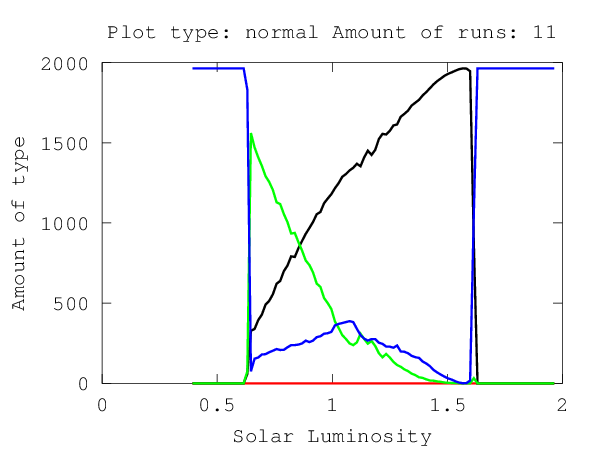
\includegraphics[width=0.4\textwidth]{../sim/output/normal}}
  \hfill
  \subfloat{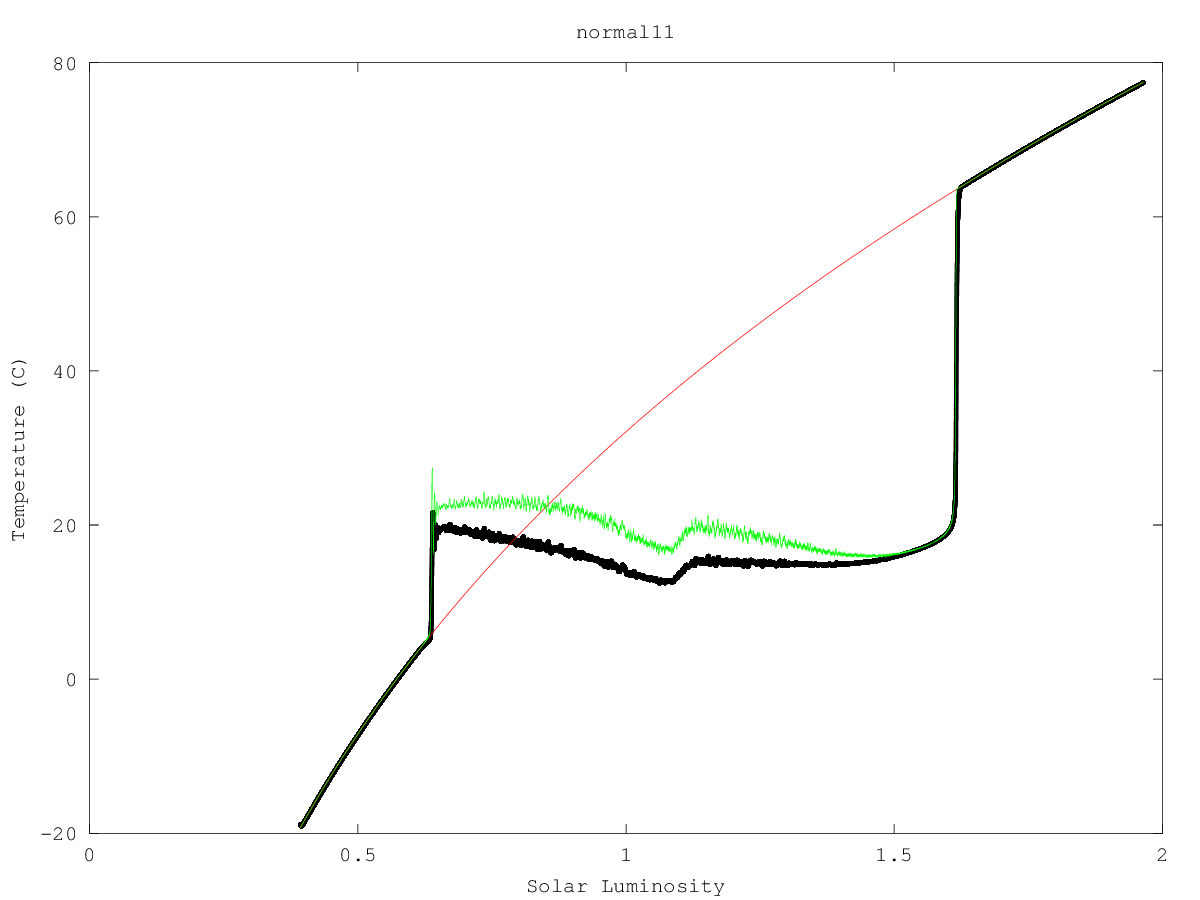
\includegraphics[width=0.4\textwidth]{../sim/output/normal-avg}}
  \caption{Normal simulation}
\end{figure}

\begin{figure}[H]
  \centering
  \subfloat{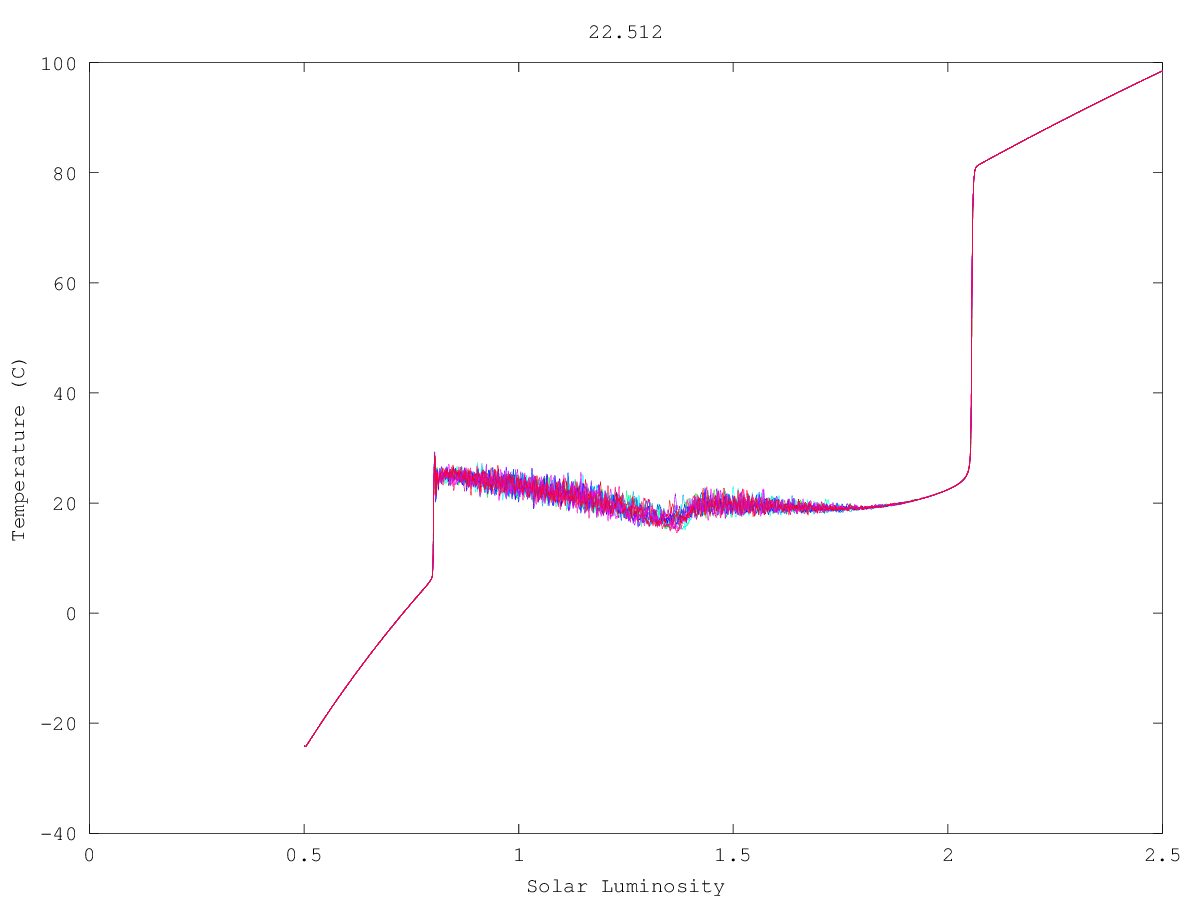
\includegraphics[width=0.4\textwidth]{{{../sim/output/22.5}}}}
  \hfill
  \subfloat{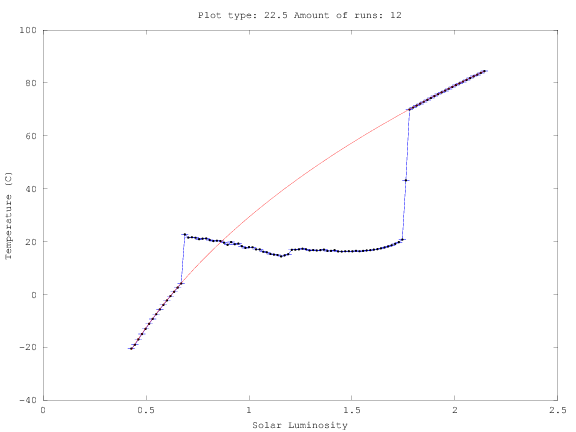
\includegraphics[width=0.4\textwidth]{{{../sim/output/22.5-avg}}}}
  \caption{Simulation with invasive blacks at 22.5 degrees}
\end{figure}

\begin{figure}[H]
  \centering
  \subfloat{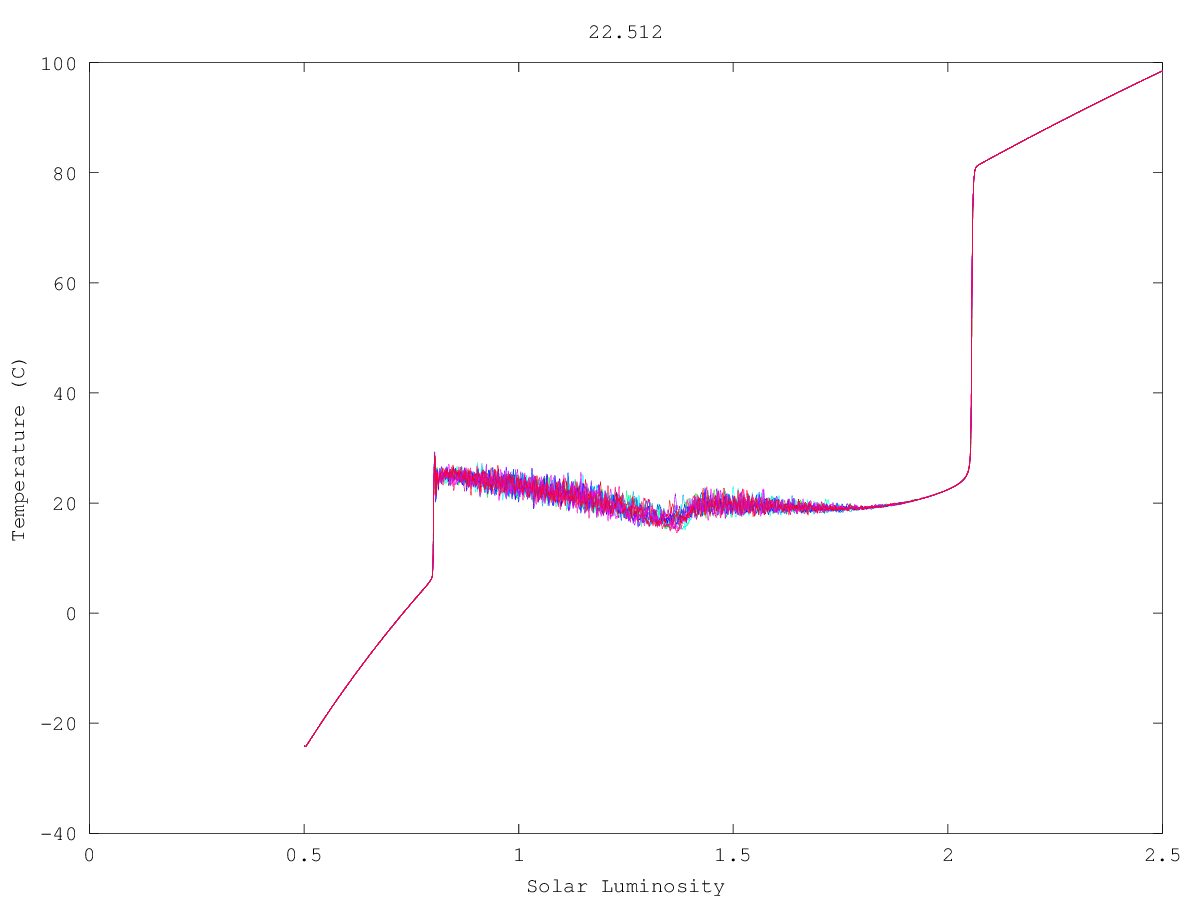
\includegraphics[width=0.4\textwidth]{{{../sim/output/22.5}}}}
  \hfill
  \subfloat{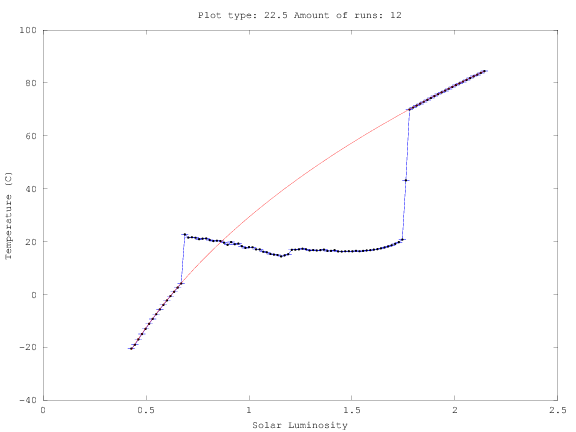
\includegraphics[width=0.4\textwidth]{{{../sim/output/22.5-avg}}}}
  \caption{Simulation with invasive blacks at 22.5 degrees}
\end{figure}

\begin{figure}[H]
  \centering
  \subfloat{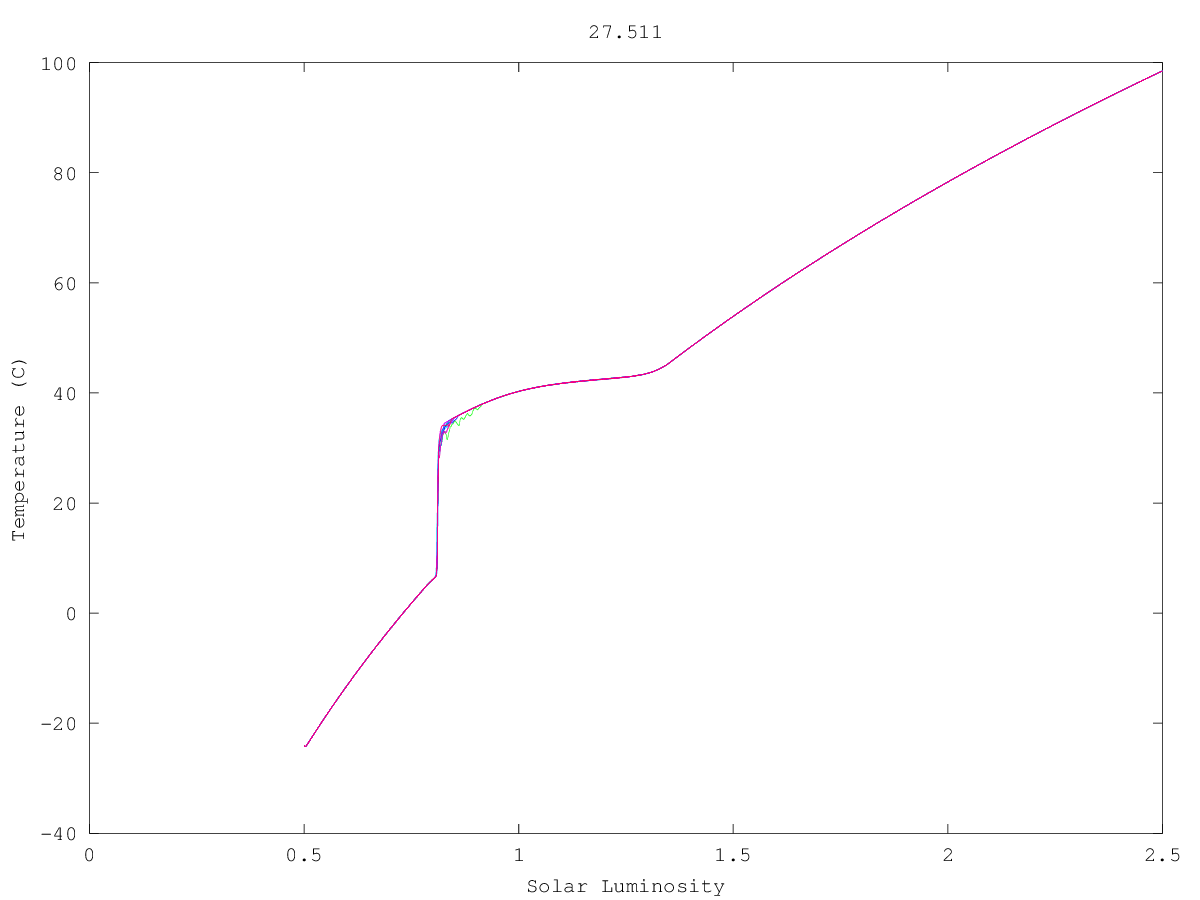
\includegraphics[width=0.4\textwidth]{{{../sim/output/27.5}}}}
  \hfill
  \subfloat{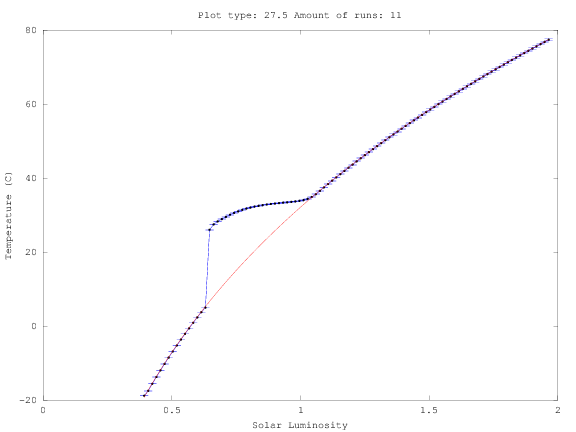
\includegraphics[width=0.4\textwidth]{{{../sim/output/27.5-avg}}}}
  \caption{Simulation with invasive blacks at 27.5 degrees}
\end{figure}

\begin{figure}[H]
  \centering
  \subfloat{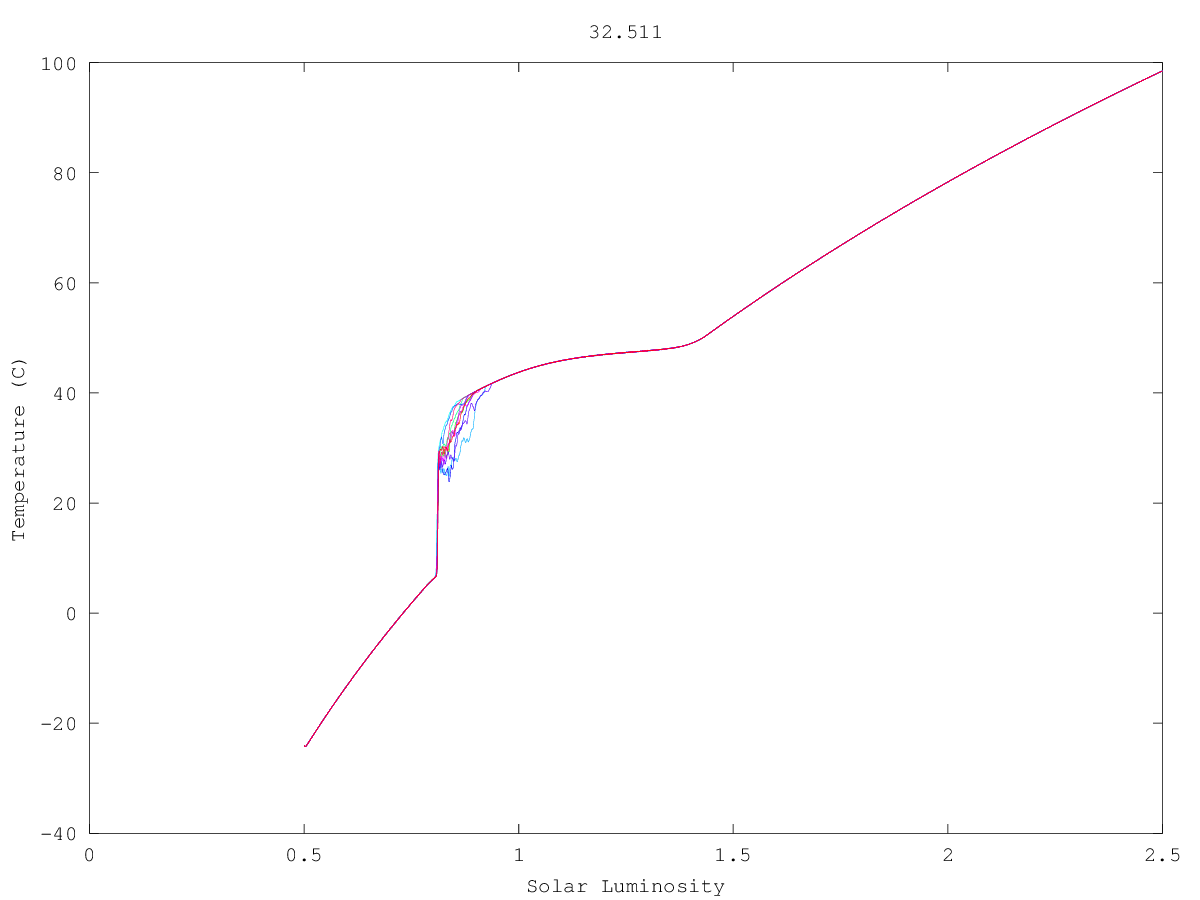
\includegraphics[width=0.4\textwidth]{{{../sim/output/32.5}}}}
  \hfill
  \subfloat{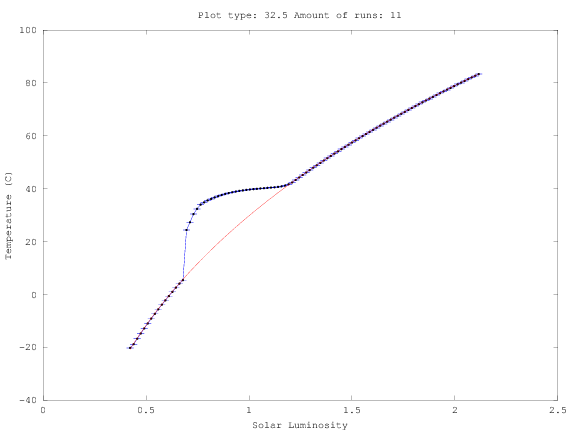
\includegraphics[width=0.4\textwidth]{{{../sim/output/32.5-avg}}}}
  \caption{Simulation with invasive blacks at 32.5 degrees}
\end{figure}

\begin{figure}[H]
  \centering
  \subfloat{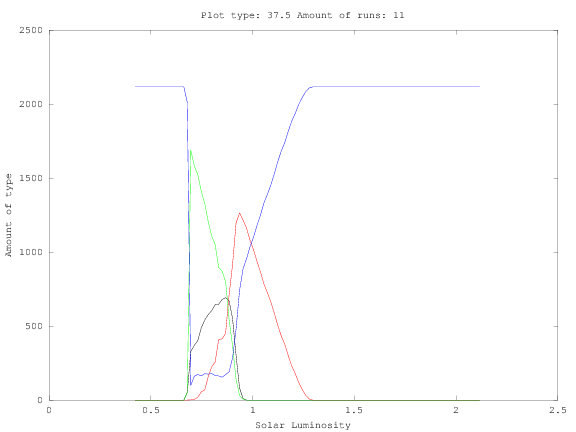
\includegraphics[width=0.4\textwidth]{{{../sim/output/37.5}}}}
  \hfill
  \subfloat{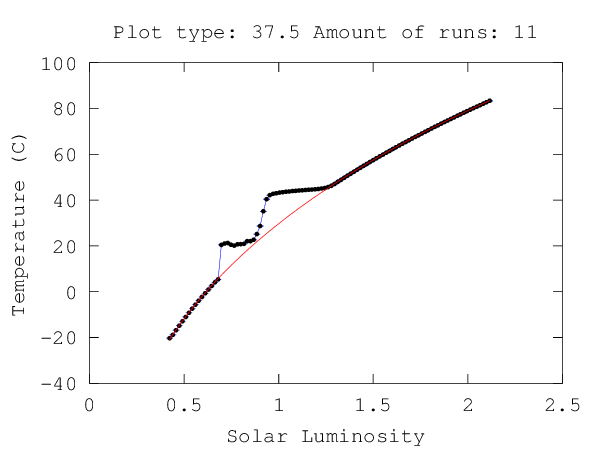
\includegraphics[width=0.4\textwidth]{{{../sim/output/37.5-avg}}}}
  \caption{Simulation with invasive blacks at 37.5 degrees}
\end{figure}

\begin{figure}[H]
  \centering
  \subfloat{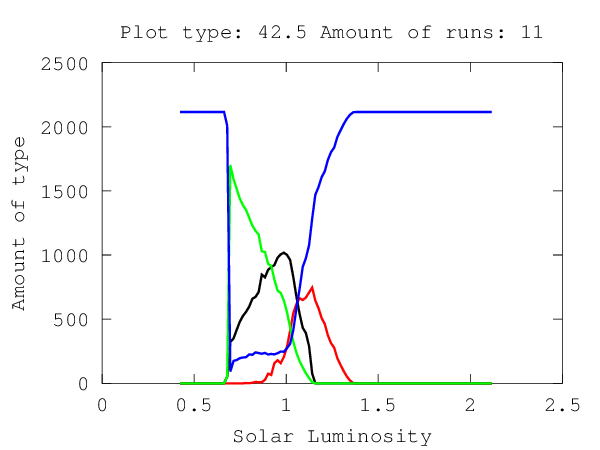
\includegraphics[width=0.4\textwidth]{{{../sim/output/42.5}}}}
  \hfill
  \subfloat{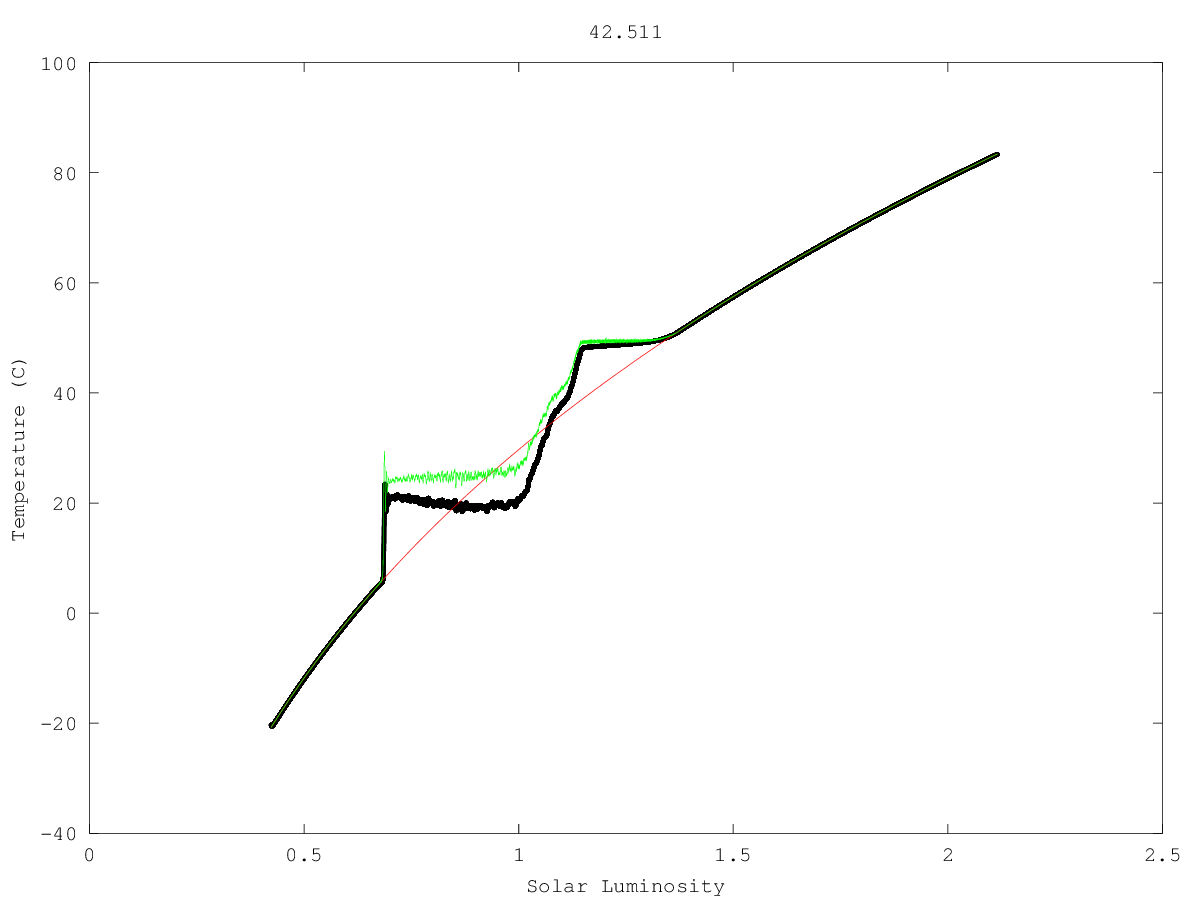
\includegraphics[width=0.4\textwidth]{{{../sim/output/42.5-avg}}}}
  \caption{Simulation with invasive blacks at 42.5 degrees}
\end{figure}

\begin{figure}[H]
  \centering
  \subfloat{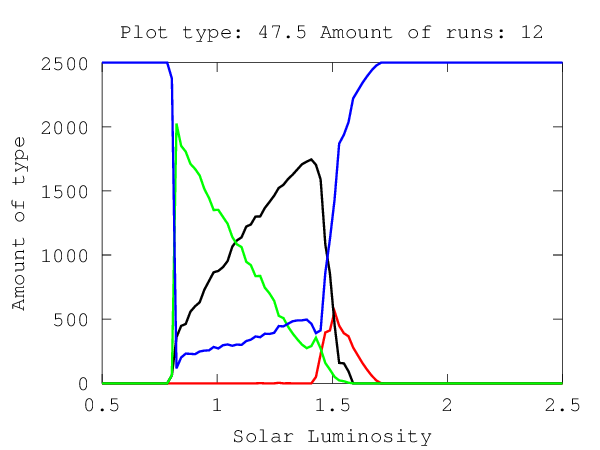
\includegraphics[width=0.4\textwidth]{{{../sim/output/47.5}}}}
  \hfill
  \subfloat{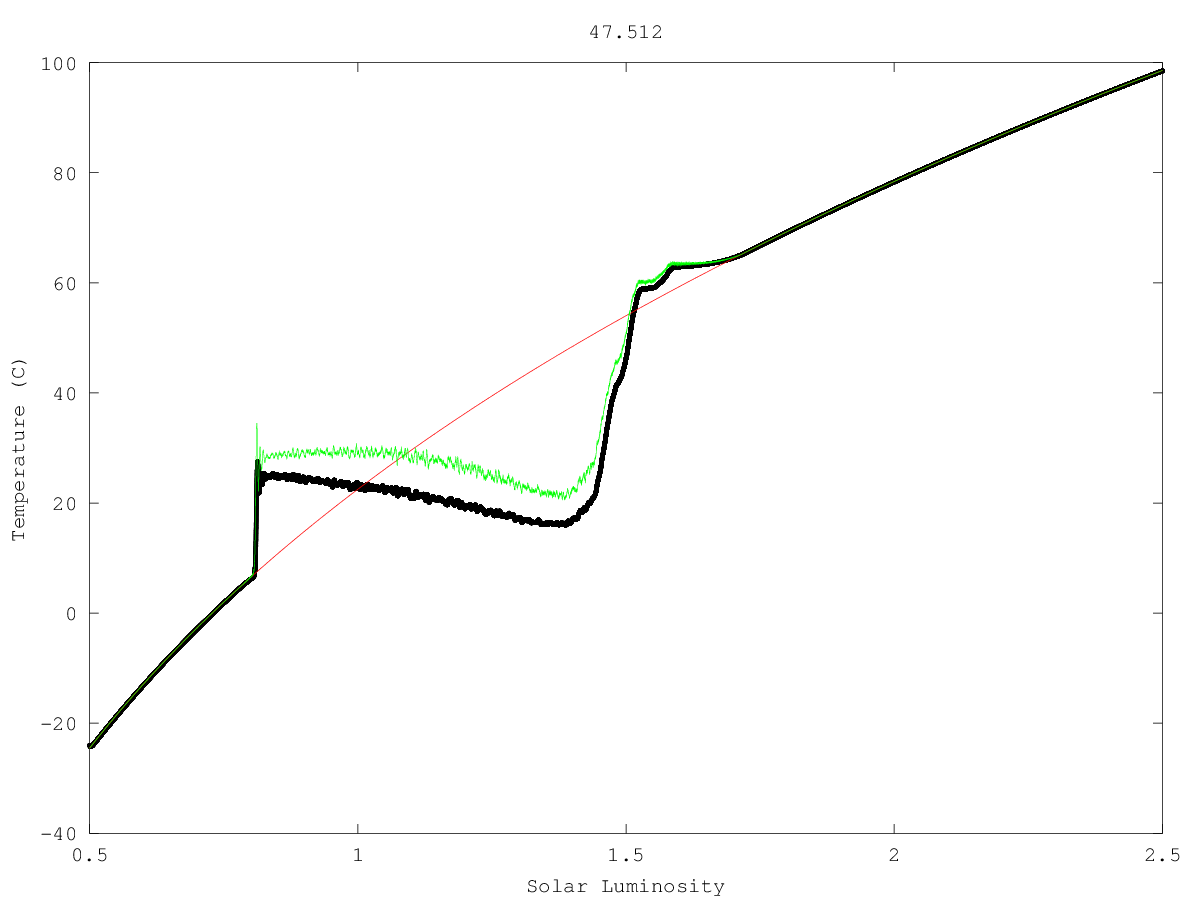
\includegraphics[width=0.4\textwidth]{{{../sim/output/47.5-avg}}}}
  \caption{Simulation with invasive blacks at 47.5 degrees}
\end{figure}

\begin{figure}[H]
  \centering
  \subfloat{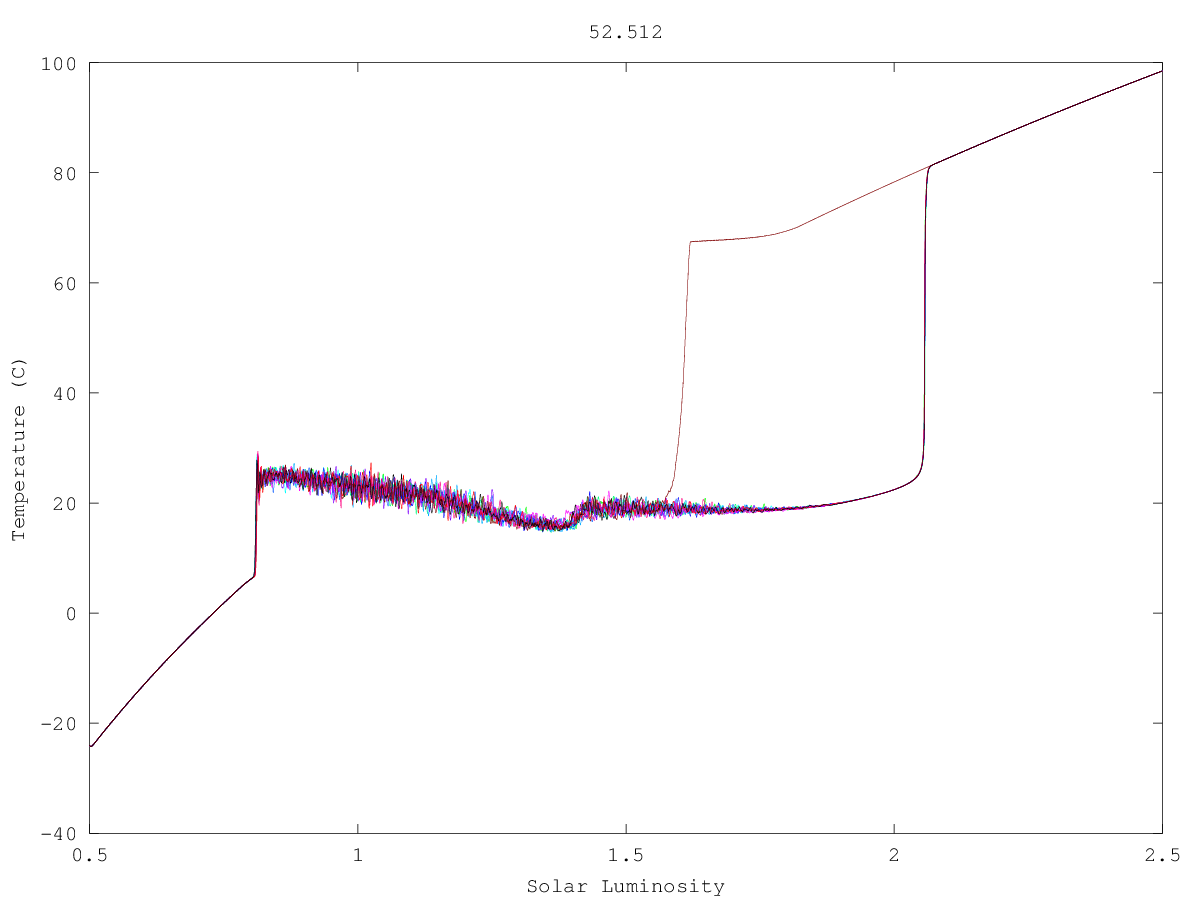
\includegraphics[width=0.4\textwidth]{{{../sim/output/52.5}}}}
  \hfill
  \subfloat{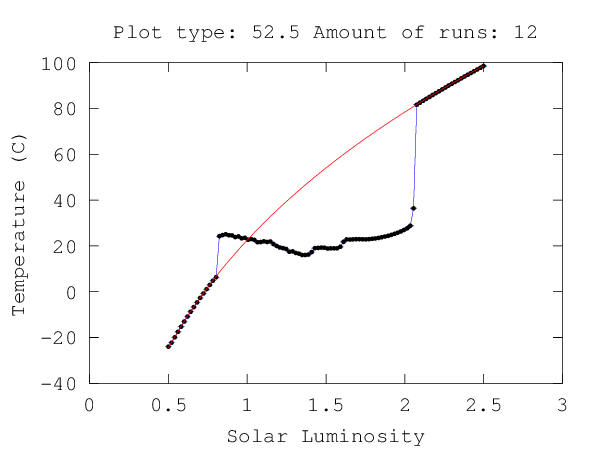
\includegraphics[width=0.4\textwidth]{{{../sim/output/52.5-avg}}}}
  \caption{Simulation with invasive blacks at 52.5 degrees}
\end{figure}

\begin{figure}[H]
  \centering
  \subfloat{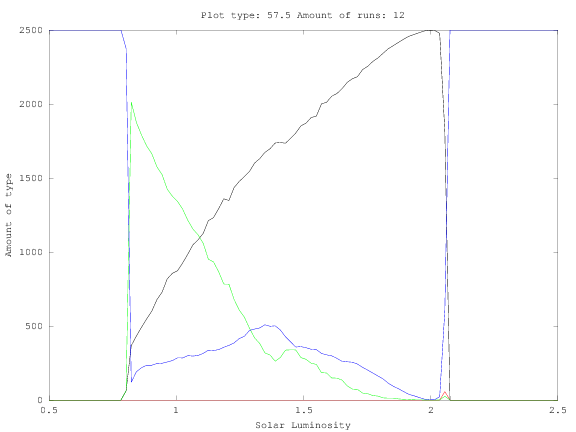
\includegraphics[width=0.4\textwidth]{{{../sim/output/57.5}}}}
  \hfill
  \subfloat{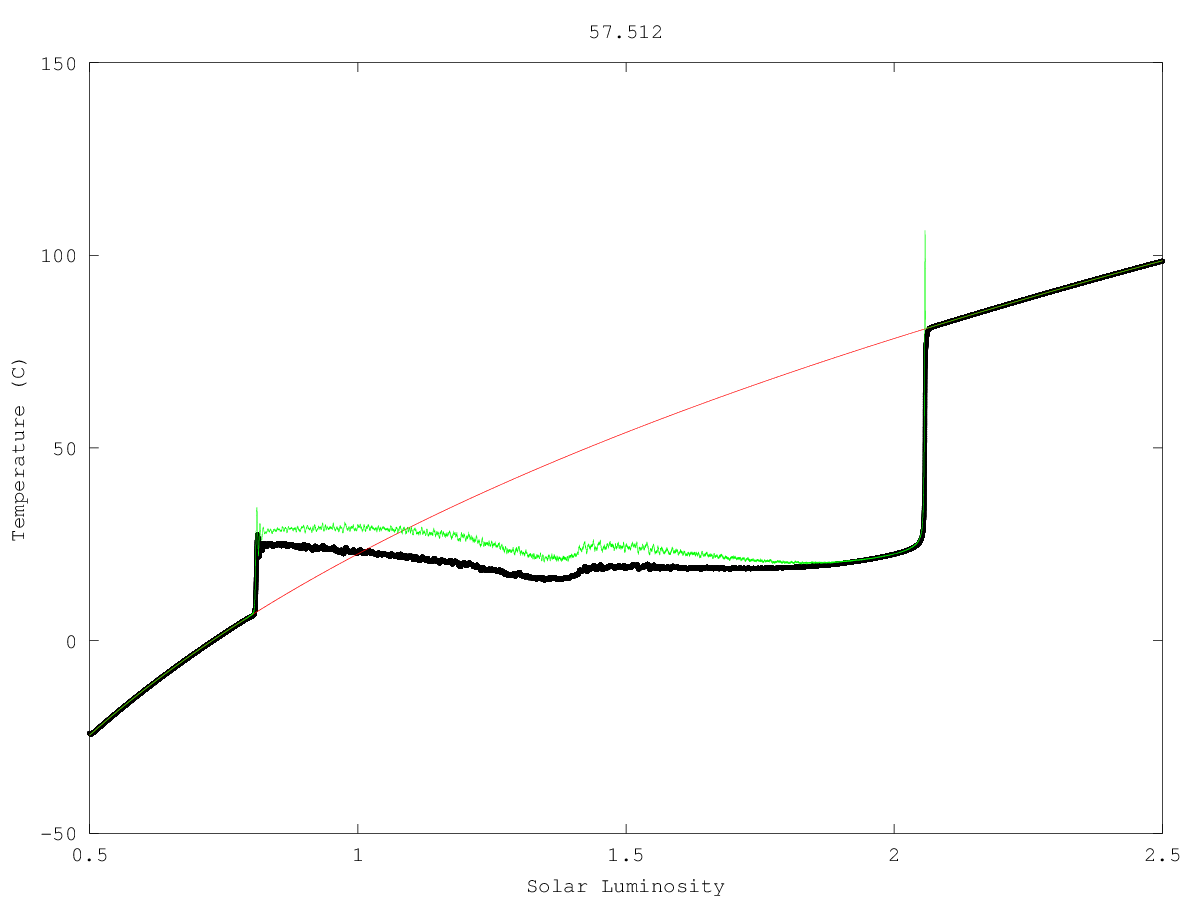
\includegraphics[width=0.4\textwidth]{{{../sim/output/57.5-avg}}}}
  \caption{Simulation with invasive blacks at 57.5 degrees}
\end{figure}


% TODO: Describe collection of results
%  - Make sure that amount of runs is shown under each diagram
%  - Show amount
%  - consider plotting amount of runs vs temp
%  - binary search for grabbing data?

\section{Analysis \& Discussion}
There seem to be three behaviours of the system with these parameters:
\begin{itemize}
\item Maintained homeostasis
\item Immediate homeostasis breakdown
\item Held-off homeostasis breakdown
\end{itemize}

These are explored in the following sections.

\subsection{Maintained homeostasis}
When the introduced species is extremely similar, or extremely
dissimilar, to the native species, homeostasis is maintained. This
could be the result of either of two cases:
\subsubsection{Extreme similarity}
The similarity between the introduced species and the natives means
that all species are attempting to keep their environment at the same
temperature (or close enough to maintain homeostasis). This can be
seen in graphs with optimal growing temperature of 22.5 to 25.5
degrees Celsius.

\subsubsection{Extreme dissimilarity}
The dissimilarity between the native species and the introduced means
that the new species never actually gets to grow at any stage when the
system is in homeostasis. The parameters that exhibit this behaviour
is 54.5 degrees Celsius and upwards.

Some analysis of the optimal growing temperature and it's range fully
explains this behaviour. Since the native daisies can only grow in the
range of $22.5 \pm 17.5$ degrees, the upper temperature limit of 40
degrees is very much below the 54.5 degrees where this behaviour starts.
\subsection{Immediate homeostasis breakdown}
This is seen in optimal growing temperatures 26.5 to 31.5 degrees
Celsius. An explanation of this is that when the system first attempts
to establish homeostasis the invasive daisies take over immediately
and quickly make the environment too hot for the natives.

The initial establishment of homeostasis is not a valid state of an
ecosystem on earth in current times, hence this region is a candidate
for further exploration, although it may be very similar to the next Sexton.

\subsection{Held-off homeostasis breakdown}
This is a very interesting region, occurring in the temperature range
of 32.5 to 53.5 degrees Celsius. Homeostasis is established, but as
the sun grows hotter and forces the system to adapt, the invasive
species takes hold and breaks homeostasis.

This mirrors ecosystems on earth, where an environment that would
normally be able to fend off an invasive species cannot due to
external stresses\cite{albert2000}.

\section{Future work}
A more in depth exploration of the three regions (especially the
``Held-off homeostasis breakdown'' and the ``Immediate Homeostasis
breakdown'') regions. Specifically:
\begin{itemize}
\item What conditions are required for the invasive species to take hold
\item Why does the system sometimes not collapse for the same
  parameters, what is the difference?
\item How does the invasive species actually take hold?
\item How much of the world is required to be invasive species before
  homeostasis breaks down?
\item What would the difference be for a invasive species that cools a
  warming daisyworld as opposed to warming it?
\end{itemize}

\section{Conclusion}
A healthy ecosystem that may normally be able to
withstand an invasive species can succumb when put under excessive
stress, such as climate change. This simulation exhibits behaviour
similar to ecosystem breakdown in these conditions. Hence it may be
an effective tool in the future exploration of the effects of ecosystem
collapse due to the introduction of invasive species.


% \section{Formatting Citations}

% Citations can be handled in one of three ways.  The most
% straightforward (albeit labor-intensive) would be to hardwire your
% citations into your \LaTeX\ source, as you would if you were using an
% ordinary word processor.  Thus, your code might look something like
% this:


% \begin{quote}
% \begin{verbatim}
% However, this record of the solar nebula may have been
% partly erased by the complex history of the meteorite
% parent bodies, which includes collision-induced shock,
% thermal metamorphism, and aqueous alteration
% ({\it 1, 2, 5--7\/}).
% \end{verbatim}
% \end{quote}


% \noindent Compiled, the last two lines of the code above, of course, would give notecalls in {\it Science\/} style:

% \begin{quote}
% \ldots thermal metamorphism, and aqueous alteration ({\it 1, 2, 5--7\/}).
% \end{quote}

% Under the same logic, the author could set up his or her reference list as a simple enumeration,

% \begin{quote}
% \begin{verbatim}
% {\bf References and Notes}

% \begin{enumerate}
% \item G. Gamow, {\it The Constitution of Atomic Nuclei
% and Radioactivity\/} (Oxford Univ. Press, New York, 1931).
% \item W. Heisenberg and W. Pauli, {\it Zeitschr.\ f.\
% Physik\/} {\bf 56}, 1 (1929).
% \end{enumerate}
% \end{verbatim}
% \end{quote}

% \noindent yielding

% \begin{quote}
% {\bf References and Notes}

% \begin{enumerate}
% \item G. Gamow, {\it The Constitution of Atomic Nuclei and
% Radioactivity\/} (Oxford Univ. Press, New York, 1931).
% \item W. Heisenberg and W. Pauli, {\it Zeitschr.\ f.\ Physik} {\bf 56},
% 1 (1929).
% \end{enumerate}
% \end{quote}

% That's not a solution that's likely to appeal to everyone, however ---
% especially not to users of B{\small{IB}}\TeX\ \cite{inclme}.  If you
% are a B{\small{IB}}\TeX\ user, we suggest that you use the
% \texttt{Science.bst} bibliography style file and the
% \texttt{scicite.sty} package, both of which we are downloadable from our author help site
% (http://www.sciencemag.org/about/authors/prep/TeX\_help/).  You can also
% generate your reference lists by using the list environment
% \texttt{\{thebibliography\}} at the end of your source document; here
% again, you may find the \texttt{scicite.sty} file useful.

% Whether you use B{\small{IB}}\TeX\ or \texttt{\{thebibliography\}}, be
% very careful about how you set up your in-text reference calls and
% notecalls.  In particular, observe the following requirements:

% \begin{enumerate}
% \item Please follow the style for references outlined at our author
%   help site and embodied in recent issues of {\it Science}.  Each
%   citation number should refer to a single reference; please do not
%   concatenate several references under a single number.
% \item Please cite your references and notes in text {\it only\/} using
%   the standard \LaTeX\ \verb+\cite+ command, not another command
%   driven by outside macros.
% \item Please separate multiple citations within a single \verb+\cite+
%   command using commas only; there should be {\it no space\/}
%   between reference keynames.  That is, if you are citing two
%   papers whose bibliography keys are \texttt{keyname1} and
%   \texttt{keyname2}, the in-text cite should read
%   \verb+\cite{keyname1,keyname2}+, {\it not\/}
%   \verb+\cite{keyname1, keyname2}+.
% \end{enumerate}

% \noindent Failure to follow these guidelines could lead
% to the omission of the references in an accepted paper when the source
% file is translated to Word via HTML.

% \section{Handling Math, Tables, and Figures}

% Following are a few things to keep in mind in coding equations,
% tables, and figures for submission to {\it Science}.

% \paragraph*{In-line math.}  The utility that we use for converting
% from \LaTeX\ to HTML handles in-line math relatively well.  It is best
% to avoid using built-up fractions in in-line equations, and going for
% the more boring ``slash'' presentation whenever possible --- that is,
% for \verb+$a/b$+ (which comes out as $a/b$) rather than
% \verb+$\frac{a}{b}$+ (which compiles as $\frac{a}{b}$).  Likewise,
% HTML isn't tooled to handle certain overaccented special characters
% in-line; for $\hat{\alpha}$ (coded \verb+$\hat{\alpha}$+), for
% example, the HTML translation code will return [\^{}$(\alpha)$].
% Don't drive yourself crazy --- but if it's possible to avoid such
% constructs, please do so.  Please do not code arrays or matrices as
% in-line math; display them instead.  And please keep your coding as
% \TeX-y as possible --- avoid using specialized math macro packages
% like \texttt{amstex.sty}.

% \paragraph*{Displayed math.} Our HTML converter sets up \TeX\
% displayed equations using nested HTML tables.  That works well for an
% HTML presentation, but Word chokes when it comes across a nested
% table in an HTML file.  We surmount that problem by simply cutting the
% displayed equations out of the HTML before it's imported into Word,
% and then replacing them in the Word document using either images or
% equations generated by a Word equation editor.  Strictly speaking,
% this procedure doesn't bear on how you should prepare your manuscript
% --- although, for reasons best consigned to a note \cite{nattex}, we'd
% prefer that you use native \TeX\ commands within displayed-math
% environments, rather than \LaTeX\ sub-environments.

% \paragraph*{Tables.}  The HTML converter that we use seems to handle
% reasonably well simple tables generated using the \LaTeX\
% \texttt{\{tabular\}} environment.  For very complicated tables, you
% may want to consider generating them in a word processing program and
% including them as a separate file.

% \paragraph*{Figures.}  Figure callouts within the text should not be
% in the form of \LaTeX\ references, but should simply be typed in ---
% that is, \verb+(Fig. 1)+ rather than \verb+\ref{fig1}+.  For the
% figures themselves, treatment can differ depending on whether the
% manuscript is an initial submission or a final revision for acceptance
% and publication.  For an initial submission and review copy, you can
% use the \LaTeX\ \verb+{figure}+ environment and the
% \verb+\includegraphics+ command to include your PostScript figures at
% the end of the compiled PostScript file.  For the final revision,
% however, the \verb+{figure}+ environment should {\it not\/} be used;
% instead, the figure captions themselves should be typed in as regular
% text at the end of the source file (an example is included here), and
% the figures should be uploaded separately according to the Art
% Department's instructions.


% \section{What to Send In}

% What you should send to {\it Science\/} will depend on the stage your manuscript is in:

% \begin{itemize}
% \item {\bf Important:} If you're sending in the initial submission of
%   your manuscript (that is, the copy for evaluation and peer review),
%   please send in {\it only\/} a PostScript or PDF version of the
%   compiled file (including figures).  Please do not send in the \TeX\
%   source, \texttt{.sty}, \texttt{.bbl}, or other associated files with
%   your initial submission.  (For more information, please see the
%   instructions at our Web submission site,
%   http://www.submit2science.org/ .)
% \item When the time comes for you to send in your revised final
%   manuscript (i.e., after peer review), we require that you include
%   all source files and generated files in your upload.  Thus, if the
%   name of your main source document is \texttt{ltxfile.tex}, you
%   need to include:
% \begin{itemize}
% \item \texttt{ltxfile.tex}.
% \item \texttt{ltxfile.aux}, the auxilliary file generated by the
%   compilation.
% \item A PostScript file (compiled using \texttt{dvips} or some other
%   driver) of the \texttt{.dvi} file generated from
%   \texttt{ltxfile.tex}, or a PDF file distilled from that
%   PostScript.  You do not need to include the actual \texttt{.dvi}
%   file in your upload.
% \item From B{\small{IB}}\TeX\ users, your bibliography (\texttt{.bib})
%   file, {\it and\/} the generated file \texttt{ltxfile.bbl} created
%   when you run B{\small{IB}}\TeX.
% \item Any additional \texttt{.sty} and \texttt{.bst} files called by
%   the source code (though, for reasons noted earlier, we {\it
%     strongly\/} discourage the use of such files beyond those
%   mentioned in this document).
% \end{itemize}
% \end{itemize}

% % Your references go at the end of the main text, and before the
% % figures.  For this document we've used BibTeX, the .bib file
% % scibib.bib, and the .bst file Science.bst.  The package scicite.sty
% % was included to format the reference numbers according to *Science*
% % style.


% \bibliography{scibib}

% \bibliographystyle{Science}



% % Following is a new environment, {scilastnote}, that's defined in the
% % preamble and that allows authors to add a reference at the end of the
% % list that's not signaled in the text; such references are used in
% % *Science* for acknowledgments of funding, help, etc.

% \begin{scilastnote}
% \item We've included in the template file \texttt{scifile.tex} a new
% environment, \texttt{\{scilastnote\}}, that generates a numbered final
% citation without a corresponding signal in the text.  This environment
% can be used to generate a final numbered reference containing
% acknowledgments, sources of funding, and the like, per {\it Science\/}
% style.
% \end{scilastnote}




% For your review copy (i.e., the file you initially send in for
% evaluation), you can use the {figure} environment and the
% \includegraphics command to stream your figures into the text, placing
% all figures at the end.  For the final, revised manuscript for
% acceptance and production, however, PostScript or other graphics
% should not be streamed into your compliled file.  Instead, set
% captions as simple paragraphs (with a \noindent tag), setting them
% off from the rest of the text with a \clearpage as shown  below, and
% submit figures as separate files according to the Art Department's
% instructions.


% \clearpage

% \noindent {\bf Fig. 1.} Please do not use figure environments to set
% up your figures in the final (post-peer-review) draft, do not include graphics in your
% source code, and do not cite figures in the text using \LaTeX\
% \verb+\ref+ commands.  Instead, simply refer to the figure numbers in
% the text per {\it Science\/} style, and include the list of captions at
% the end of the document, coded as ordinary paragraphs as shown in the
% \texttt{scifile.tex} template file.  Your actual figure files should
% be submitted separately.


\begin{thebibliography}{99}
  \bibitem{morgan2001}
    Ernest, S. and Brown, J. (2001). Homeostasis and Compensation: The
    Role of Species and Resources in Ecosystem Stability. Ecology,
    82(8), p.2118.

  \bibitem{barry2014} Barry, G. (2014). Terrestrial ecosystem loss
    and biosphere collapse. Management of Env Quality, 25(5), pp.542-563.

\bibitem{rapport1985}
  Rapport, D., Regier, H. and Hutchinson, T. (1985). Ecosystem
  Behavior Under Stress. The American Naturalist, 125(5), p.617.

\bibitem{watson1983}
  Watson, A.~J. and J.~E. Lovelock, 1983: Biological homeostasis of the global
  environment: the parable of daisyworld. {\em Tellus}, {\bf 35B},
  284--289.
\bibitem{gilbert2007}
  Gilbert, G. (n.d.). Agent-based models.

\bibitem{albert2000}
Alpert, P., Bone, E. and Holzapfel, C. (2000). Invasiveness, invasibility and the role of environmental stress in the spread of non-native plants. Perspectives in Plant Ecology, Evolution and Systematics, 3(1), pp.52-66.

\end{thebibliography}


\end{document}




















